\documentclass[11.5pt]{article}
\usepackage[utf8]{inputenc}
\usepackage[T1]{fontenc}
\usepackage[textwidth=460pt, top=80pt, bottom=80pt]{geometry}
\usepackage{graphicx}
\usepackage[justification=default]{subfig}
\usepackage[update]{epstopdf}
\usepackage[labelfont=bf]{caption}
\usepackage[dvipsnames]{xcolor}
\usepackage{fancyhdr}
\usepackage{booktabs}
\usepackage{multicol}
\usepackage{multirow}
\usepackage{titling}
\usepackage{float}
\usepackage{bm}
\usepackage[intlimits]{empheq}
\usepackage[hidelinks]{hyperref}
\usepackage{amsmath}
\usepackage{csquotes}
\usepackage{enumitem}
\usepackage{tikz}
\usetikzlibrary{positioning, 3d}
\usepackage{tabularx}

%Bibliography

\usepackage{csquotes}
\usepackage[
    sorting=none, %
    sortcites=true, %
    bibencoding=ascii, %
    autopunct=true, %
    hyperref=true, %
    language=auto, %
    %backref=true,%
    url=false, %
    %maxcitenames=10,%
    %minbibnames = 20,%
    maxbibnames=3, %
    giveninits,
    natbib=false,
    isbn=false, %
    backend=biber
]{biblatex}
\addbibresource{bibliography.bib}

\usepackage[]{hyperref}
\usepackage{cleveref}
%%% CREF setup
\crefname{equation}{Eq.}{Eqs.}
\crefname{table}{Table}{Tables}
\crefname{figure}{Fig.}{Figs.}

\begin{document}
    \begin{titlingpage}
        \begin{center}
            \begin{figure}
                \centering
                
\includegraphics[width=0.6\textwidth]{
                    graphics/logo.png
                }
            \end{figure}
            \Large{\textsc{Politecnico di Milano}}
            \vspace{1cm}
            \rule{0.95\textwidth}{0.7mm}
            {\Large{\textbf{Requirement Engineering and Design Project:\\ SustainCity \\ V 1.0.1}}}
            \rule{0.95\textwidth}{0.7mm}
            \vspace{1cm}
            \large{Authors: \\ \textbf{Riccardo Donati, Camilo Martínez, Jialiclaudio Huang, Peng Rao}}

            \vspace{1cm}
            
            \text{Last update: \today}
            % \large{Authors: \\ \textbf{Peng Rao} (ID 270661)}
        \end{center}
    \end{titlingpage}

    \pagenumbering{roman}

    \tableofcontents

    \clearpage

    \setcounter{page}{1}
    \pagenumbering{arabic}

    \section{The Project and Project Goals}
    
    \subsection{Introduction}
    Urban commuting represents a significant contributor to environmental degradation and climate change, generating substantial air pollution and greenhouse gas emissions. The \textbf{SustainCity} project addresses this critical challenge through an intelligent software system designed to optimize urban traffic management and public transport operations, thereby reducing transportation's environmental footprint.
    
    \subsection{Project Overview}
    The SustainCity system synthesizes three key data streams:
    \begin{itemize}
        \item Real-time traffic sensor measurements
        \item Public transport timetables
        \item Event scheduling information
    \end{itemize}
    This integration enables dynamic traffic flow adjustments while proposing sustainable long-term optimizations. The solution leverages existing urban infrastructure combined with automated decision-making algorithms to balance operational efficiency with environmental sustainability.
    
    \subsection{Problem Statement}
    Current urban commuting patterns require mitigation through three coordinated intervention types:
    \begin{enumerate}
        \item \textbf{Dynamic Traffic Light Adjustment (Type1)}: Automatically modulate traffic light durations on arterial roads using real-time congestion data. For instance, extending green phases for dominant traffic flows while temporarily restricting cross traffic during peak periods.
        
        \item \textbf{Traffic Pattern Optimization (Type2)}: Systematically analyze daily traffic trends to recommend structural improvements including:
        \begin{itemize}
            \item One-way road configurations
            \item Traffic light schedule optimizations
            \item Public transport timetable synchronization
        \end{itemize}
        
        \item \textbf{Event-Driven Management (Type3)}: Anticipate crowd movements through event schedules (e.g., concerts, sports events) to implement preemptive adjustments in:
        \begin{itemize}
            \item Traffic light patterns
            \item Road access restrictions
            \item Public transport capacity allocation
        \end{itemize}
    \end{enumerate}
    
    \subsection{Supporting Infrastructure}
    The system architecture integrates three core components:
    \begin{itemize}
        \item \textbf{Traffic Sensor Network}: Event-driven sensors publishing intersection wait times via message bus (AMQP/MQTT)
        \item \textbf{Public Transport API}: Microservice providing timetable data through:
        \begin{itemize}
            \item \texttt{getScheduleByStreet(streetName)}
            \item \texttt{getScheduleByLine(lineNumber)}
        \end{itemize}
        \item \textbf{Event Feed}: RSS/API integration with municipal event calendars
    \end{itemize}
    
    \subsection{Stakeholders}
    \begin{itemize}
        \item \textbf{Urban Traffic Managers}: Authorize and implement Type2/3 recommendations through the city's traffic control system
        \item \textbf{Transport Operators}: Adjust fleet schedules based on system-generated predictive models
        \item \textbf{Citizens}: Access transparent reporting on traffic policies and environmental impact metrics
        \item \textbf{Event Organizers}: Provide scheduling data through municipal coordination channels
    \end{itemize}
    
    \subsection{Technical Objectives}
    The project implementation focuses on three primary deliverables:
    \begin{itemize}
        \item \textbf{Real-Time Control System}:
        \begin{itemize}
            \item Automated execution of Type1 actions
            \item Comprehensive action logging for audit purposes
        \end{itemize}
        
        \item \textbf{Decision Support Module}:
        \begin{itemize}
            \item Type2: Generate long-term optimization proposals
            \item Type3: Create event-specific configuration plans
        \end{itemize}
        
        \item \textbf{Public Reporting Interface}:
        \begin{itemize}
            \item Daily metrics: Average traffic flow + Type1 interventions
            \item Annual reviews: Implemented vs. rejected proposals with emissions impact analysis
        \end{itemize}
    \end{itemize}
    
    \subsection{Methodological Approach}
    This project applies software engineering principles from the HPC course through:
    \begin{itemize}
        \item \textbf{Requirement Engineering}: Formal specification of:
        \begin{itemize}
            \item Use cases with actor interactions
            \item Functional \& non-functional requirements
            \item Domain constraints and assumptions
        \end{itemize}
        
        \item \textbf{Architectural Design}: Structural decomposition using:
        \begin{itemize}
            \item Component diagrams showing system modules
            \item Sequence diagrams detailing critical interactions
        \end{itemize}
        
        \item \textbf{Critical Analysis}: Identification and mitigation strategies for:
        \begin{itemize}
            \item Real-time system latency challenges
            \item Data integration complexity
            \item Fail-safe mechanism requirements
        \end{itemize}
    \end{itemize}

    \section{Requirement analysis}
    \subsection{Relevant human and non-human actors}
    \subsubsection{Human Actors}
        \begin{itemize}
        \item \textbf{Urban Area Managers}
        Approve or reject proposed traffic optimizations.
        Oversee traffic management and policy decisions.
        \item \textbf{Citizens}
        Access daily and yearly reports on traffic adjustments. 
        Stay informed about the city's traffic management.
        \end{itemize}
    \subsubsection{Non-Human Actors}
    \begin{itemize}
        \item \textbf{Traffic Sensor System}
    Collects real-time traffic data and publishes it on the message bus.
    Publishes congestion levels to the event-driven infrastructure.
    \item \textbf{Public Transport System (Microservice)}
    Provides schedule data for buses and public transport lines.
    Assists in traffic analysis and optimization planning.
    \item \textbf {News Channel}
    Publishes real-time event announcements that may impact traffic.
    \end{itemize}
    
    \subsection{Use cases}

    This section describes three use cases, each corresponding to one of the system's defined action types. Each use case includes key elements such as the involved actors, flow of events, exceptions, and special requirements, offering a detailed view of how the system manages various operational scenarios.
    
    \subsubsection{Modify Traffic Lights (Type1)}

    The Modify Traffic Lights use case enables real-time adjustment of traffic signal timings based on live congestion data from the Traffic Sensor System. When traffic accumulation is detected, the system generates and applies new light configurations to improve flow. 
    
    \begin{table}[!htp]
        \centering
        \begin{tabular}{@{} l p{23em} @{}}
            \toprule \multicolumn{2}{c}{Use Case: \textbf{Modify Traffic Lights}} \\
            \midrule                                                                          %%%
            Actors                                                                           &  Traffic Sensor System, Citizens \\
            %%%
            Entry condition                                                                  &  Traffic congestion is detected through real-time analysis, requiring traffic light adjustments.\\
            %%%
            Flow of Events                                                                   & \begin{enumerate}[left=0pt, parsep=0pt, topsep=0pt]
            \item System receives traffic data from the Traffic Sensor System.
            \item A new light timing configuration is generated based on congestion analysis.
            \item Updated timings are sent to the Traffic Light Controller.
            \item The controller applies the changes and confirms success.
            \item Changes are logged via the Logging Service.
            \item The Report Generator retrieves logs daily and creates a report including Type 1 actions.
            \end{enumerate} \\
            %%%
            Exit condition                                                                   &  New traffic light durations are applied and confirmed. \\
            %%%
            Exceptions                                                                       &  \begin{enumerate}[left=0pt, parsep=0pt, topsep=0pt]
            \item Communication failure when retrieving or applying the configuration.
            \item Invalid configuration (e.g., unsafe green light duration).
            \item Logging service is unavailable.
            \end{enumerate} \\
            Special Requirements                                                             & \begin{enumerate}[left=0pt, parsep=0pt, topsep=0pt]
            \item All changes must be securely logged
            \item Communication must be encrypted.
            \item System must operate with high availability and near real-time response.
            \end{enumerate} \\
            \bottomrule
        \end{tabular}
        \caption{Detailed use case Modify Traffic Lights.}
        \label{Use Case - Research Trip}
    \end{table}
    \subsubsection{Type2}
    \begin{table}[!htp]
        \centering
        \begin{tabular}{@{} l p{23em} @{}}
            \toprule \multicolumn{2}{c}{Use Case: \textbf{Dynamic Traffic Light Adjustments}} \\
            \midrule                                                                          %%%
            Actors                                                                           &  \\
            %%%
            Entry condition                                                                  &  \\
            %%%
            Flow of Events                                                                   &  \\
            %%%
            Exit condition                                                                   &  \\
            %%%
            Exceptions                                                                       &  \\
            Special Requirements                                                             &  \\
            \bottomrule
        \end{tabular}
        \caption{Detailed use case explanation - Research Trip.}
        \label{Use Case - Research Trip}
    \end{table}

    \newpage
    
    \subsubsection{Event-Specific Traffic Configuration(Type 3)}
    This use case details how the \textbf{SustainCity system} collects information about planned large crowd events and defines event-specific configurations for traffic lights, roads and public transport schedules. 

    \begin{table}[H]
        \centering
        \begin{tabular}{@{} l p{23em} @{}}
            \toprule \multicolumn{2}{c}{Use Case: \textbf{Define Event-Specific Traffic Configurations}} \\
            \midrule   
            \textbf{Actors} & News Channel, SustainCity System, Urban Area Managers \\
            \textbf{Entry condition} & A planned event (e.g., concert, sports game) is announced via the news channel. \\
            \textbf{Flow of Events} & 
            \begin{enumerate}[left=0pt, parsep=0pt, topsep=0pt]
              \item The system receives an event notification from the city news channel.
              \item It extracts key details: type, location, timing, and expected attendance.
              \item Affected streets and areas are identified.
              \item Public transport schedules for those areas are retrieved via the microservice.
              \item Recent and historical traffic data is analyzed.
              \item Based on the analysis, the system generates event-specific configuration suggestions:
              \begin{itemize}
                \item Adjust traffic lights
                \item Modify road directions
                \item Update public transport schedules
              \end{itemize}
              \item Suggestions are sent to urban area managers.
              \item All suggestions and their acceptance status are logged for reporting.
            \end{enumerate}
             \\
            \textbf{Exit condition} & Event-specific traffic configurations are implemented or rejected. \\
            \textbf{Exceptions} & 
            \begin{itemize}[left=0pt, parsep=0pt, topsep=0pt]
                \item News Channel Feed is unavailable: The system attempts to reconnect to the News Channel Feed every 5 minutes.
                \item Event attendance significantly exceeds predictions: The system triggers an emergency traffic pattern reconfiguration
            \end{itemize} \\
            \textbf{Special Requirements} & 
            \begin{itemize}[left=0pt, parsep=0pt, topsep=0pt]
                \item System must respond to event notifications in near real-time.
                \item Generated suggestions must be traceable for yearly reporting.
                \item Suggestions must be explainable and visualizable for city officials.
            \end{itemize} \\
            \bottomrule
        \end{tabular}
    \end{table}
    
    \subsection{Domain Assumptions}
    The system design relies on the following foundational premises:
    
    \paragraph{Data Quality \& Infrastructure}
    \begin{itemize}
        \item \textbf{Sensor Accuracy}: Traffic sensors maintain ±2\% measurement accuracy for vehicle wait times under normal operating conditions
        \item \textbf{Message Bus Reliability}: The event bus (AMQP/MQTT) guarantees at-least-once delivery for sensor data with $\le$ 1s latency
        \item \textbf{API Stability}: Public transport microservice maintains backward\-compatible API versions for $\ge$ 6 months after updates
    \end{itemize}
    
    \paragraph{System Availability}
    \begin{itemize}
        \item \textbf{Microservice Uptime}: Critical external services (transport API, event feed) maintain 99.9\% monthly availability
        \item \textbf{Network Continuity}: Municipal networks provide $\ge$ 100Mbps bandwidth for real-time control commands
        \item \textbf{Power Infrastructure}: Traffic light systems have redundant power supplies with $\le$ 5s failover time
    \end{itemize}
    
    \paragraph{Stakeholder Behavior}
    \begin{itemize}
        \item \textbf{Manager Responsiveness}: Urban managers review/reject Type2/3 proposals within 48h (95\% of cases)
        \item \textbf{Event Reporting}: Venues submit event details (location, time, capacity) $\ge$ 72h before start time
        \item \textbf{Transport Punctuality}: Public transport adheres to schedules with $\le$ 5min deviation in 90\% of daily trips
    \end{itemize}
    
    \paragraph{Operational Context}
    \begin{itemize}
        \item \textbf{Traffic Light Control}: Municipal infrastructure accepts API-based phase adjustments within 30s latency
        \item \textbf{Event Impact Window}: Crowd-generated congestion remains localized within 1km of event venues
        \item \textbf{Reporting Latency}: Citizen-facing dashboards reflect data with $\le$ 15min delay for time-sensitive metrics
    \end{itemize}
    
    \noindent\textit{These assumptions form boundary conditions for system operation. Violations would trigger fallback procedures outlined in the fault tolerance specification.}
    
    \subsection{Requirements}
    \subsubsection{Functional Requirements}
    
    \paragraph{Type 1: Real-Time Traffic Control}
    \begin{itemize}
        \item \textbf{Data Acquisition:} Interface with traffic sensor network to ingest real-time intersection wait times via message bus
        \item \textbf{Congestion Detection:} Analyze traffic flow patterns using sliding window algorithms (15s intervals) to identify bottlenecks
        \item \textbf{Adaptive Signal Control:} Dynamically adjust traffic light phases based on:
        \begin{itemize}
            \item Relative traffic density across connected roads
            \item Priority thresholds (e.g., +25\% volume triggers extended green phase)
            \item Minimum/maximum phase duration constraints
        \end{itemize}
        \item \textbf{Action Logging:} Maintain tamper-evident logs of all signal adjustments with timestamp, location, and duration changes
        \item \textbf{Public Reporting:} Generate daily PDF/JSON reports containing:
        \begin{itemize}
            \item Hourly traffic flow averages per arterial road
            \item Summary of signal interventions (frequency, duration, locations)
        \end{itemize}
    \end{itemize}
    
    \paragraph{Type 2: Strategic Traffic Optimization}
    \begin{itemize}
        \item \textbf{Historical Analysis:} Process 30-day traffic patterns using time-series clustering to identify recurrent congestion hotspots
        \item \textbf{Configuration Proposals:} Generate optimization plans including:
        \begin{itemize}
            \item One-way street conversions (with estimated flow improvement \%)
            \item Traffic light timing presets for different day periods
            \item Public transport schedule adjustments (±15min windows)
        \end{itemize}
        \item \textbf{Approval Workflow:} Provide web interface for urban managers to:
        \begin{itemize}
            \item Review proposals with cost/benefit projections
            \item Approve/reject with mandatory justification comments
        \end{itemize}
        \item \textbf{Decision Audit:} Maintain versioned records of all proposals and responses
    \end{itemize}
    
    \paragraph{Type 3: Event-Driven Management}
    \begin{itemize}
        \item \textbf{Event Ingestion:} Subscribe to municipal event calendars via iCal/RSS feeds
        \item \textbf{Impact Simulation:} Predict traffic disruptions using:
        \begin{itemize}
            \item Venue capacity data
            \item Historical attendance patterns
            \item Public transport access points
        \end{itemize}
        \item \textbf{Mitigation Planning:} Auto-generate contingency plans featuring:
        \begin{itemize}
            \item Temporary road closures/reroutes
            \item Public transport capacity boosts (+30\% vehicles)
            \item Parking restriction zones
        \end{itemize}
        \item \textbf{Approval Chain:} Require multi-level authorization for major changes:
        \begin{itemize}
            \item Traffic manager (road modifications)
            \item Transit director (schedule changes)
        \end{itemize}
    \end{itemize}
    
    \subsubsection{Non-Functional Requirements}
    \begin{itemize}
        \item \textbf{Performance:}
        \begin{itemize}
            \item Process sensor updates within 500ms (p95 latency)
            \item Execute signal adjustments within 2s of decision trigger
            \item Support 1M+ daily sensor events at peak load
        \end{itemize}
        
        \item \textbf{Availability:}
        \begin{itemize}
            \item 99.99\% uptime for critical control subsystems
            \item Hot standby redundancy for signal adjustment module
        \end{itemize}
        
        \item \textbf{Scalability:}
        \begin{itemize}
            \item Linear horizontal scaling for data ingestion layer
            \item Support city expansion up to 5000 intersections
        \end{itemize}
        
        \item \textbf{Security:}
        \begin{itemize}
            \item RBAC with OAuth2.0 for management interfaces
            \item End-to-end encryption for all control commands
            \item Annual penetration testing requirements
        \end{itemize}
        
        \item \textbf{Usability:}
        \begin{itemize}
            \item Web dashboard with SLA of 2s page load time
            \item Multi-language support for citizen reports
            \item A11y-compliant interfaces (WCAG 2.1 AA)
        \end{itemize}
    \end{itemize}
    
    \noindent\textit{These requirements directly support the project's three core intervention types while addressing operational constraints identified in stakeholder analysis.}

    \newpage
    \section{Design}
    \subsection{General description of the architecture}
    \subsection{Sequence diagrams}
    \subsubsection{Type1}
    Description of the main elements of the Type1 sequence diagram:
    \begin{enumerate}
        \item Participants
        \begin{itemize}
        \item \textbf{Traffic Sensor System (TSS):} Represents the sensor infrastructure that collects real-time traffic data.  
        \item \textbf{Traffic Management System (TMS):} It is the central system that processes the data from the sensors. It is responsible for analyzing traffic flow, detecting congestion, and deciding actions for adjusting traffic light timings. It also manages some statistics for reporting purposes.
        \item \textbf{Traffic Light Controller (TLC):} It is the controller for managing the traffic lights. Once the TMS determines if an action of adjusting traffic light durations is needed, it sends instructions to the TLC. The controller then updates the lights configuration and confirms the update back.
        \item \textbf{Logging Service:} It is responsible for logging any changes made to traffic light durations.
        \item \textbf{Report Generator:} It fetches the necessary logs and stats from the TMS and generates the reports. This includes daily statistics on traffic flow and the actions taken by the system.
        \item \textbf{Citizen Platform:} Provides access to traffic reports for citizens.
    \end{itemize}

    \item Interactions
        \begin{itemize}
        \item \textbf{publishTrafficData():} The Traffic Sensor System sends real-time traffic data to the Traffic Management System (TMS).
        \item \textbf{analyzeTrafficFlow():} The TMS processes the received traffic data. This step involves analyzing the flow of traffic, calculating statistics like vehicle counts, wait times, and traffic density.
        \item \textbf{evaluateCongestionPatterns():} After analyzing traffic flow, the TMS evaluates the data to detect congestion patterns. For example, if the traffic density exceeds a predefined threshold, the system decides whether action is needed, such as extending green lights.
        \item \textbf{updateLightConfig(roadId, newConfig):} Based on the congestion patterns, the TMS instructs the Traffic Light Controller (TLC) to update the duration of the traffic lights on specific roads. For example, it may decide to extend the green light on a busy road.
        \item \textbf{confirmUpdate():} The TLC confirms that the traffic light timings have been updated successfully.
        \item \textbf{logAction(updatedDetails):} The TMS logs the change details to the Logging Service.
        \item \textbf{fetchLogs():} The Report Generator fetches the logs from the Logging Service to gather all recorded actions for that day.
        \item \textbf{getTrafficStats():} The Report Generator retrieves the necessary traffic statistics from the TMS. 
        \item \textbf{generateDailyStats():} The Report Generator processes the logs and stats to generate the daily traffic report about the average traffic flow on the main roads.
        \item \textbf{displayDailyReport():} The Report Generator publishes the daily report to the Citizen Platform, where it is made available for public viewing.
    \end{itemize}
    \end{enumerate}

    \begin{figure}[htbp]
        \centering
        \includegraphics[width=0.9\textwidth]{figures/sequence-diagram-type1.pdf}
        \caption{Type1 sequence diagram.}
        \label{fig:sequence-diagram-type1}
    \end{figure}
    
    \subsubsection{Type2}

    \newpage
    
    \subsubsection{Type3}
    \begin{figure}[htbp]
        \centering
        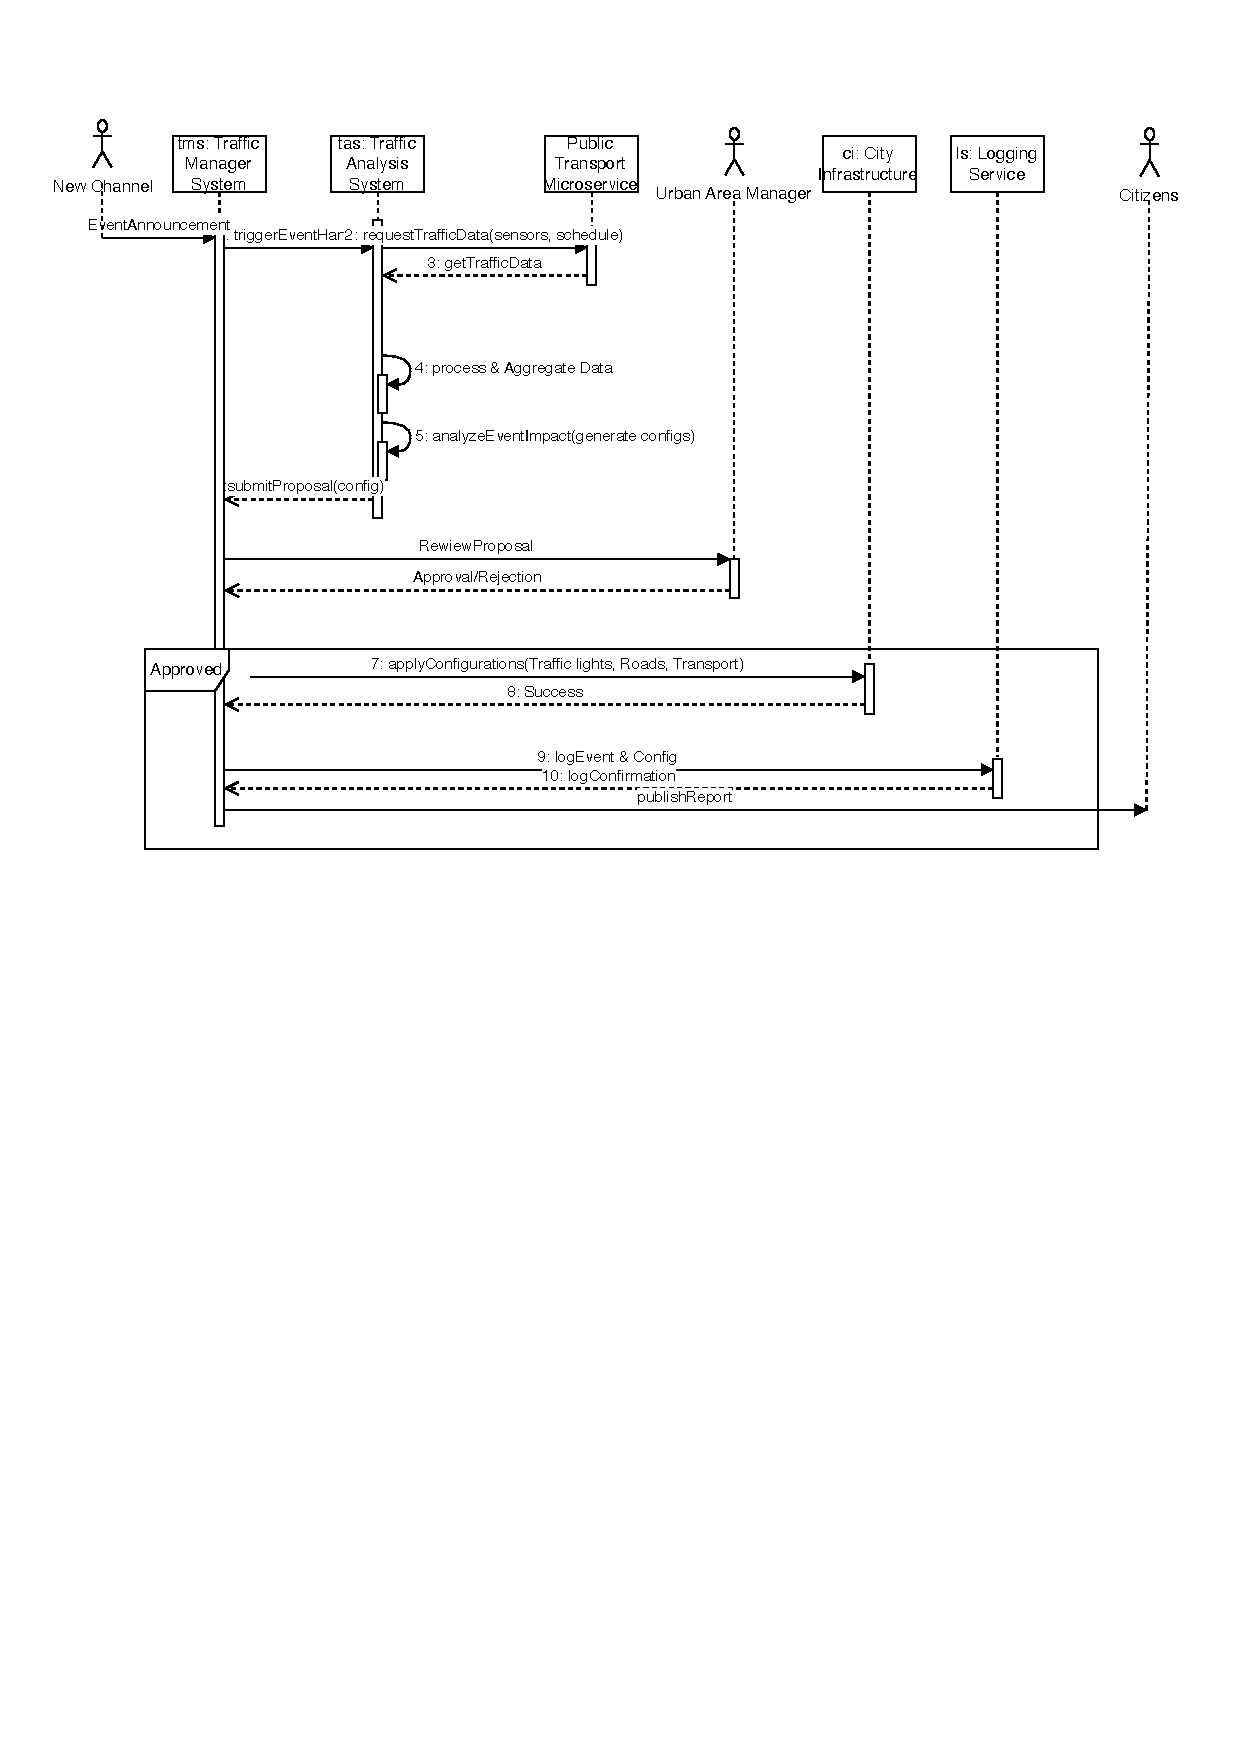
\includegraphics[width=0.9\textwidth]{figures/sequence-diagram-type3.pdf}
    \end{figure}
    \par{Participants:}
    \begin{itemize}
        \item \textbf{News Channel}: Publishes event announcements (e.g., concerts, sports events) as soon as they are planned.
        \item \textbf{Traffic Management System}: The central system managing the entire process.
        \item \textbf{Traffic Analysis System}: Responsible for data processing and traffic impact analysis.
        \item \textbf{Public Transport Microservice}: Provides real-time data from public transport (buses, metros, etc.).
        \item \textbf{Urban Area Managers}: Responsible for reviewing and approving proposed traffic plans.
        \item \textbf{City Infrastructure}: The actual infrastructure (e.g., traffic lights, roads) that will apply changes.
        \item \textbf{Logging Service}: Stores logs of events and configurations.
    \end{itemize}
    The main interactions could be as follows:
    \begin{enumerate}
        \item \textbf{Event Announcement}. News Channel $\rightarrow$ Traffic Management System: Sends EventNotification(eventDetails) (asynchronous message). The news channel transmits event details (e.g. location, time, expected crowd size).
        \item \textbf{Fetch Public Transport Data}. 
        \begin{itemize}
            \item Traffic Analysis System $\rightarrow$ Public Transport Microservice: Calls getScheduleByStreet(streetName) (synchronous).
            \item Public Transport Microservice $\rightarrow$ Traffic Analysis System: Returns ScheduleData.
        \end{itemize}
        \item \textbf{Generate Configuration Plan}. Traffic Analysis System $\rightarrow$ Traffic Analysis System: GenerateConfigurationPlan() (self-message). Processes event data and transport schedules to create traffic light adjustments, road changes, and public transport updates.
        \item \textbf{Suggest Configuration to Managers} Traffic Analysis System $\rightarrow$ Urban Area Managers: Sends SuggestConfiguration(configurationPlan). Proposes event-specific changes (e.g., extend green lights on main routes, set one-way roads).
        \item \textbf{Manager Approval}. Urban Area Managers $\rightarrow$ Traffic Management System: Sends ApprovalResponse(approved). Managers review and approve the plan (assumed approval for this flow).
        \item \textbf{Apply Traffic Light Configurations}. Traffic Management System $\rightarrow$ City Infrastructure: Sends ApplyTrafficLightConfig(config).
        \item \textbf{Log Action and Update Reports}. Traffic Manager System $\rightarrow$ Logging Service: Sends LogType3Action(config, "Applied"). Records the action for yearly reports and citizen notifications.
    \end{enumerate}

    \subsection{Critical Points and Design Decisions}
    
    The SustainCity system's complexity and real-time demands introduce several critical challenges. Below are the key considerations and corresponding design resolutions:
    
    \begin{itemize}
        \item \textbf{Real-Time Data Processing}
        \begin{itemize}
            \item \textbf{Criticality}: Sensor data must be processed in real time to adjust traffic lights (Type1 actions) without latency
            \item \textbf{Design Decisions}: 
            \begin{itemize}
                \item Event-driven architecture using Apache Kafka for high-throughput sensor data ingestion
                \item \textbf{HPC-optimized stream processing} with Apache Flink, leveraging parallel computing for multi-intersection analysis
                \item GPU-accelerated traffic prediction models for congestion threshold calculations
            \end{itemize}
        \end{itemize}
    
        \item \textbf{System Reliability}
        \begin{itemize}
            \item \textbf{Criticality}: Downtime could disrupt traffic management and public safety
            \item \textbf{Design Decisions}:
            \begin{itemize}
                \item \textbf{Distributed HPC framework} using Kubernetes with MPI integration for fault-tolerant parallel processing
                \item \textbf{Data replicatio}n across HPC nodes using Hadoop Distributed File System (HDFS)
                \item Cloud auto-scaling with AWS Batch for compute-intensive tasks
            \end{itemize}
        \end{itemize}
    
        \item \textbf{HPC Workload Management}
        \begin{itemize}
            \item \textbf{Criticality}: Balancing compute-intensive and data-intensive workloads
            \item \textbf{Design Decisions}:
            \begin{itemize}
                \item \textbf{Hybrid HPC architecture}: 
                \begin{itemize}
                    \item Compute nodes with high-core CPUs for traffic simulations (Type2/Type3)
                    \item Data nodes with NVMe storage for real-time sensor processing (Type1)
                \end{itemize}
                \item \textbf{Dynamic resource partitioning} using Slurm workload manager
                \item \textbf{In-memory computing} with Apache Ignite for frequent-access traffic patterns
            \end{itemize}
        \end{itemize}
    
        \item \textbf{Large-Scale Data Processing}
        \begin{itemize}
            \item \textbf{Criticality}: Annual report generation requires petabyte-scale historical analysis
            \item \textbf{Design Decisions}:
            \begin{itemize}
                \item \textbf{MapReduce implementation} for distributed aggregation of yearly traffic data
                \item \textbf{Columnar storage} using Parquet format for efficient archival/retrieval
                \item \textbf{Federated learning} across edge nodes to reduce central system load
            \end{itemize}
        \end{itemize}
    
        \item \textbf{Complex Traffic Simulations}
        \begin{itemize}
            \item \textbf{Criticality}: City-wide simulations require massive parallel computing
            \item \textbf{Design Decisions}:
            \begin{itemize}
                \item \textbf{MPI-based parallelization} of traffic flow algorithms across HPC clusters
                \item \textbf{CUDA-optimized microsimulations} for individual vehicle behavior modeling
                \item \textbf{Approximate computing} techniques for near-real-time scenario testing
            \end{itemize}
        \end{itemize}
    \end{itemize}
    
    The architecture combines HPC paradigms with cloud-native design, using MPI/OpenMP for compute-intensive tasks (traffic simulations, ML models) and Spark/Flink for data-intensive operations (sensor streams, reporting). \textbf{Hybrid HPC scheduling} ensures optimal resource allocation between batch-oriented Type2 analyses and real-time Type1 adjustments.
    
    \clearpage
    \printbibliography
    [heading=bibintoc, title = {References}]
\end{document}